\chapter{Self-host化したSwiftコンパイラの設計と実装}
\label{implementation}

本章では、本研究で現行のコンパイラとその実行部分LOCを比較するSelf-host化したSwiftコンパイラに必要な設計について述べ、実装について紹介する。

\section{評価に必要な実装範囲の検討}
\label{implementation:refinement}

~\ref{issue:barometer}節でも述べたように、Swiftコンパイラは非常に大きなソフトウェアであるため、評価結果から適切な考察を行うためには、これをより小さな部分に分け、部分ごとに評価を行う必要がある。
そのために同節では本研究における可読性を表す指標として実行部分LOCを使用することを説明したが、それによって特定のプログラムを対象とした時に必要となるコンパイラの部分だけを取り出したとしても、その中に含まれる処理には多数のステップがあり、まだ適切な考察を行うために十分対象を切り分けられているとはいえない。

また、Self-host化したSwiftコンパイラと現行のSwiftコンパイラの実行部分LOCを比較した際に、その差がSelf-host化によって生まれたものであると考えるためには、2つのコンパイラの比較箇所においてSelf-host化以外の大きな実装上の差があってはならない。
しかし、Self-host化したSwiftコンパイラではそもそも実装に同様の手法を用いることができない処理ステップも存在しうる。

そこで本研究では、現行のSwiftコンパイラをその機能によっていくつかの部分に切り分けた上で、各部分における目的と使用されている手法についてまとめ、その部分をSelf-host化した場合でも同じ目的のもとに同様の手法を取ることが可能かどうかを考察した上で、特に比較を行う上で有意義だと思われる一部分についてのみ、現行のSwiftコンパイラと同等の機能を持つように実装する。

\section{現行のSwiftコンパイラの構成}
\label{refinement:structure}

Swiftコンパイラの大まかな構成を図~\ref{img:swift-compiler-process}に示した。
この図はSwiftの中心的開発者であるGroffとLattnerによるSwiftコンパイラについての説明資料~\cite{sil}中の図を訳し簡略化したものである。
Swiftコンパイラは図中矩形で表されている5つの処理によって図中円形で表されている4つのデータ形式を順に読み込み・生成する。
データ形式から処理を貫いて他のデータ形式まで伸びる矢線はデータ形式がどの処理によってどの順に生成されるかを表している。

\begin{figure}
    \begin{center}
        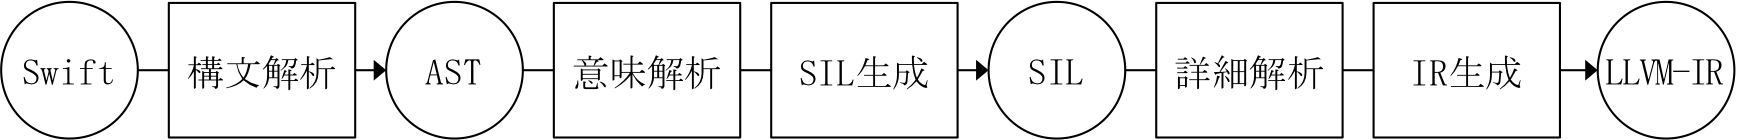
\includegraphics[scale=0.5]{./img/swift_compiler_process.png}
        \caption{Swiftコンパイラの構成}
        \label{img:swift-compiler-process}
    \end{center}
\end{figure}

この図が表現しているのは、Swiftコンパイラのデータ構造を媒介とした各処理ステップの独立性である。
Swiftコンパイラでは各処理ステップで扱うデータ形式を原則としてSwift、AST、SIL、LLVM-IRのいずれかに限定することで処理ステップ間の結合を疎にしている。

以下ではSwiftコンパイラで行われる各処理ステップについて、それぞれの目的とそのために使用されている手法について概説する。
なお、本論文内のSwiftコンパイラについての説明はswift-2.2-SNAPSHOT-2015-12-31-aのリリースにおける構成に基づいている。

\subsection{構文解析}
\label{refinement:structure:parser}

構文解析は次の2つの目的のために行われる。

\begin{enumerate}
    \item ただの文字列であるSwiftプログラムを解析して構造を持った抽象構文木(AST)に変換する
    \item プログラムの構文的な誤りを検知して報告する
\end{enumerate}

1つ目の目的を達成するために、SwiftではLL(k)クラスの再帰下降構文解析を手作業で構築して用いている。
この手法についての理解を深めるために、以下では近代的なプログラミング言語に用いられるもう1つの構文解析手法と共にこの構文解析手法について解説する ~\cite{dragonbook}。

\subsubsection{下向き構文解析}

下向き構文解析では、プログラム全体を表現する非終端記号の文法から順により詳細な構成要素に深さ優先で分解していくことによってプログラムを解析する。
Swiftで用いられているLL(k)クラスの再帰下降構文解析は下向き構文解析の1種である。

再帰下降構文解析は関数によって表現された手続きの集合として構成され、最初の文法を表現する手続きからより詳細な構成要素のための文法を表現する手続きを再帰的に呼び出すことで処理が行われる。
そのため、再帰下降構文解析では文法と実装が明確な対応関係を持っている事が多く、手作業で構文解析器を作成することが比較的簡単である。

\subsubsection{上向き構文解析}

上向き構文解析では、プログラムの字句を先頭から順に読み、具体的な字句をより抽象的な非終端記号へと還元していくことで当てはまる文法を決定し、プログラムを解析する。

上向き構文解析において最もよく用いられているのはLR(1)クラスの構文解析器である。
LR(1)クラスの解析器は多くのプログラミング言語で用いられる文法の殆どを解析できる上、Yaccに代表されるような古くからよく用いられている構文解析器の自動生成ソフトウェアが存在する。
ただし、逆にLR(1)クラスの解析器を手作業で記述するのは容易ではない。
なお、LL(k)クラスの解析器についても構文解析器を自動生成するソフトウェアは存在する~\cite{antlr}が、LR(1)クラスの解析器ほど頻繁に使用されてはいない。

\vspace{2em}

このように構文解析器には複数の設計手法が存在しており、その内の幾つかの手法においては同等の解析能力を保持しているが、どの手法を採用するかによって構文解析器のプログラムは大きく変化する。
また、構文解析器の2つ目の目的であるエラー検知については、その構文解析器が自動生成されるような場合には自動生成されたプログラムの用意するインターフェースによって検知タイミングや検知の難易度が変化する場合がある。

これに加えて、SwiftではSwiftで作成されたライブラリを読み込むためにCやC++におけるヘッダファイルと同じような役割を担う独自形式のモジュールファイルをライブラリ作成時に自動生成しており、構文解析器はこれを解析する役割も担っている。

\subsection{意味解析}
\label{refinement:structure:sema}

意味解析の目的は次のとおりである。

\begin{enumerate}
    \item AST中の変数や関数、型を互いに結びつけ、プログラム全体の整合性を確認する
    \item 開発者によって省略されている情報を補足する
\end{enumerate}

1つ目の目的は主に参照解決と型検査、2つ目の目的は主に型推論を行うことによって達成される。
以下では意味解析の中で行われるこれら3つの処理についてSwiftで使用されている手法について述べる。

\subsubsection{参照解決}

プログラム中で使用される変数や関数が正確にどこで宣言された変数や関数を指しているかを知ることができるタイミングはその変数や関数がどんな種類であるかに依存する。

例えば、プログラム~\ref{code:explicit-reference}のようなSwiftプログラムでは2行目で参照される変数xが直前の行で宣言されているため、構文解析を行いながら宣言された変数の情報を蓄積しておけば、最短で2行目のxを読んだ直後に変数xの参照を解決できる。
それに対してプログラム~\ref{code:implicit-reference}のように少し複雑化すると、例えばプログラム中5行目の変数s.xの参照を解決するためにはいくつかのステップを踏む必要が出てくる。
このプログラムでprint関数に渡されている関数s.fの参照を解決するためには、まず変数sの参照を解決し、その型が明示されていないためにこれを推論し、クラスSampleのメンバリストから関数fの2つの宣言を探した上で、s.fに与えられている引数の型を調べ、それがInt型であるために2つの宣言のうちInt型を引数に取る方を選ぶ、という長大なステップを踏まなければならない。

\begin{lstlisting}[caption=直ちに変数解決が可能である例, label=code:explicit-reference]
let x: Int = 1
print(x)
\end{lstlisting}

\begin{lstlisting}[caption=変数解決までに複数の処理が必要となる例, label=code:implicit-reference]
class Sample {
    func f(a: Int) {
        print("int")
    }
    func f(a: String) {
        print("string")
    }
}
let s = Sample()
print(s.f(0))
\end{lstlisting}

このように、参照解決のタイミングはプログラミング言語の仕様によって制限されるが、特に最短のタイミングで解決を行わないといけないということもないため、実装時の簡潔性などを勘案した上で実装ごとに決定される。
実際、現行のSwiftコンパイラでも参照解決のタイミングはその変数や関数の参照のされ方によってまちまちである。

\subsubsection{型検査・型推論}

SwiftはHaskellやMLなどの関数型言語と同様の非常に強力な型システムを備えており、その型検査と型推論はHindleyとMilnerによる型推論アルゴリズムを拡張したアルゴリズムによって行われている~\cite{swift-type-checker} ~\cite{tapl}。

HindleyとMilnerによる型推論アルゴリズム自体は非常によく知られている上に様々な言語で採用されているが、現行のSwiftコンパイラで行われている独自の拡張は他の型推論を用いる関数型言語と比較してSwiftに特徴的なパラダイムであるオブジェクト指向プログラミングや型パラメータ多相、関数のオーバーロードを実現するためのものであり、これらを強力な型推論アルゴリズムと共に採用している言語は極めて少ない。

\subsection{SIL生成}

SIL生成は、ASTを分析してより抽象度の低いSwift独自の中間言語であるSwift Intermediate Language(SIL)に変換することで最適化などの準備を行うためのステップである。
SILはLLVM-IRをベースとしてループやエラー処理、オブジェクト指向プログラミングのためのクラスの概念などを拡張し、プログラムの意味に基づく詳細なエラー検出などを行い易くした言語である ~\cite{sil}。

SIL生成のステップは特に一般的な手法などに基づいた処理が行われているわけではなく、完全にASTとSILの設計に依存した処理となる。

\subsection{詳細解析}
\label{refinement:structure:analyze}

詳細解析は、SILを分析してASTのような抽象度の高い状態やLLVM-IRのような抽象度の低い状態では処理しづらい最適化やエラー検出を行うためのステップである。

現行のSwiftコンパイラではSILが包含するコールグラフやクラス階層といった情報を元に最適化やエラー検出を行っており、それらは手法ごとにモジュール化されている。
また、Swiftではメモリ管理の手法として各オブジェクトの作成が要求された際に自動的にメモリを割り当て、不要になったタイミングを検知してメモリを開放するAutomatic Reference Counting方式を用いており~\cite{arc}、そのための処理の挿入などもこの詳細解析で行っている。

\subsection{IR生成}

IR生成はSILを分析してLLVM-IRを生成することで、低抽象度での最適化や機械語生成を行うための準備を行うためのステップである。

LLVMは統一された中間言語であるLLVM-IRに対する最適化やLLVM-IRから様々なプラットフォーム上で動作可能な機械語へのコンパイルを行うツール群であり~\cite{llvm}、現行のコンパイラはこのLLVMを用いることでコンパイラのバックエンドをフロントエンドから完全に分離している。

なお、LLVMのツールセットは実行可能なソフトウェアや用意されたAPIを通して使用されており、現行のコンパイラではC++で記述されたAPIを用いている。
このAPIには他の言語向けのものも存在するが、LLVMのツールは主にC++で記述されているためにC++のAPIが最も充実しており、現行のSwiftコンパイラはC++のAPIのみで実装されている高度なインターフェースを利用している。

\section{実装の概要}
\label{implementation:abstract}

本研究では、~\ref{refinement:structure}節におけるSwiftコンパイラの構成要素の観察から、構文解析器についてのみ注目し、これを実装して比較評価を行う。
同節で述べたように、各構成要素はそれぞれに比較が困難になる可能性のある箇所があるが、構文解析器はコンパイラ内で始めに実行される箇所であるために他の処理から分離しやすく、用いられている手法も明確に定義されている一般的なものである。
そのため、本研究での比較評価には構文解析器を用いる。

以降では実装したSwiftコンパイラの構文解析器について、Swiftプログラムから構文を構成する字句に分解する字句解析、字句を構文にまとめ上げる構文解析、通常のプログラムとは異なるライブラリ用のモジュールファイルを解析するモジュール解析、およびそれらで発生するエラーを処理するエラー検出の4つの処理機能に分けてその実装を紹介する。

本論文では現行のApple社によるSwiftコンパイラと簡単に区別するため、以降では本研究で実装するSwiftコンパイラを指してTreeSwift~\ref{treeswift}と記述する。
また、TreeSwiftでは完全ではないものの、構文解析器以外の部分についても実装を行い、構文解析器が充分機能するものであることを確認している。

\subsubsection{字句解析}

TreeSwiftでは字句解析を文字分類器と字句解析器の2つのモジュールによって行う。
文字分類器は図~\ref{img:character-classifier}のようにソースコードを1文字ずつ読み込み、各文字に所属する字句グループに関する注釈をつけることで、字句解析での文字の判断を補助する役割を担う。
字句解析器は注釈付きの文字を順に読み込んで、Swiftで用いられる各字句が生成できるか判断する小さなオートマトンの集まりからなっており、図~\ref{img:lexical-analyzer}のようにそれらを平行して動かすことで、後戻りなしに注釈付きの文字を字句に分割する。

\begin{figure}
    \begin{center}
        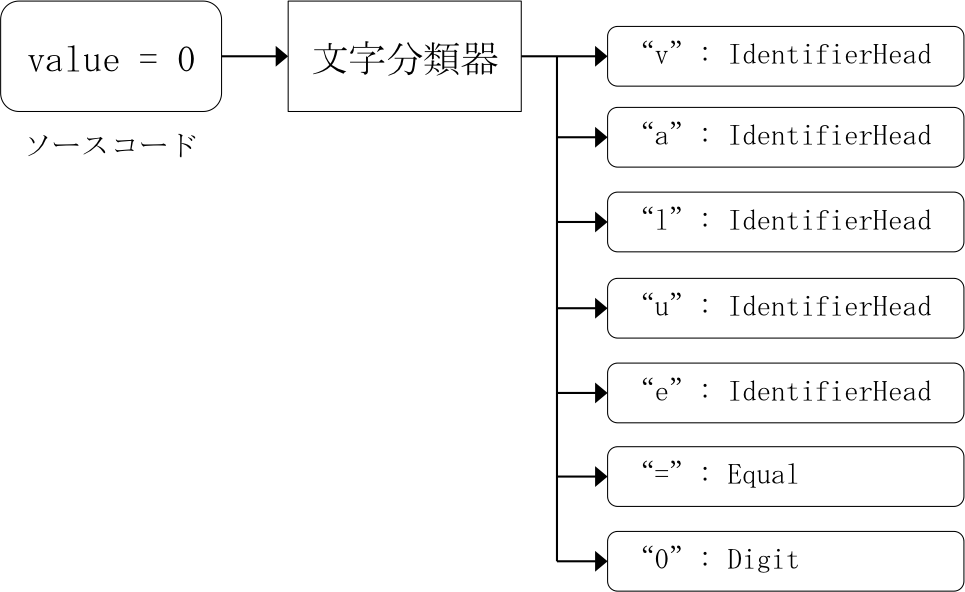
\includegraphics[scale=0.8]{./img/character_classifier.png}
        \caption{文字分類器の仕組み}
        \label{img:character-classifier}
    \end{center}
\end{figure}

\begin{figure}
    \begin{center}
        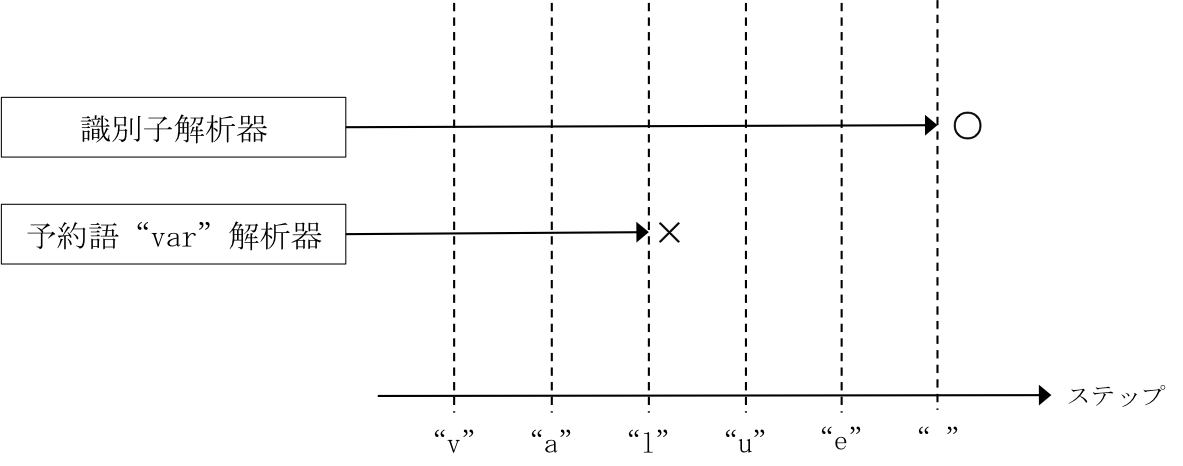
\includegraphics[scale=0.8]{./img/lexical_analyzer.png}
        \caption{字句解析器の仕組み}
        \label{img:lexical-analyzer}
    \end{center}
\end{figure}

\subsubsection{構文解析}

TreeSwiftの構文解析は~\ref{refinement:structure:parser}節で述べた現行のSwiftコンパイラと同じLL(k)クラスの再帰下降構文解析を用いている。

また、ASTに用いるデータ構造にはSwiftの特徴を活かして列挙体とクラスを使い分けることで、ASTを分解する際に実行時の型情報に基づく動的型変換の使用を避けられるように設計している。

\subsubsection{モジュール解析}

TreeSwiftでは標準ライブラリを含む外部ライブラリに定義されている変数や関数、型などに関する情報をモジュールファイルとしてコンパイラに供給することで、外部ライブラリ内で定義されている要素をimport文で取り込み、使用できるようにしている。
現行のSwiftコンパイラは同じ働きをするモジュールファイルを独自形式で提供しているが、TreeSwiftではSwiftに近い構文を持つテキストファイルを用いている。

\subsubsection{エラー検出}

TreeSwiftの構文解析器はもちろん誤った構文に対してエラーを報告するが、エラー回復を行ってできるだけ多くのエラーを検出するような動作は行っていないため、基本的には1つのエラーを検出した時点で停止してしまう。

%%% Local Variables:
%%% mode: japanese-latex
%%% TeX-master: "../bthesis"
%%% End:
